\chapter{Research Portfolio}
\label{sec:research-portfolio}
\lfoot{Research Portfolio} 
%\rfoot{Research Portfolio} 

%\begin{tcolorbox}[title=Summary of Excellence]
%My research primarily focuses on providing \emph{precise and scalable techniques} and \emph{software tools} used for engineering critical software-intensive systems with a recent focus on \emph{smart and safe cyber-physical systems} (CPS) deployed over decentralized, heterogeneous platforms. As the leader of an excellent research team with 15 PhD and 25+ Masters students I supervised or co-supervised, we received \emph{7x Best/Distinguished Paper Awards} at major peer-reviewed conferences of software engineering (3 of which since joining McGill). I also received \emph{two 10-year most influential papers} for past results achieved in my early career. My research papers received over 6700 citations yielding an h-index of 43. In the past 5 years, I was invited to deliver 6 keynote talks at international or national conferences or workshops, 10 talks at advanced schools, and 15+ talks at industrial events.
%
%\vspace{3pt}
%
%%\paragraph{A paragraph}
%Moreover, I have actively contributed to turn \emph{novel research results and prototype tools} first into \emph{industrial strength open source frameworks} then \emph{to innovative services and products} maintained by IncQuery Labs, a successful Hungarian company co-founded with my former graduate students and used by major international companies.
%% operating in the CPS domain.
%\end{tcolorbox}

\paragraph{Organization of research portfolio}

My career as an indepenent researcher consists two main stages. \textbf{Stage 1} is from 2004 when I started to independently supervise students at BME, which included 5 PhD students and numerous MSc students until 2014.
I successfully received a tenured position in 2009 and I was promoted to a full professor at BME in 2014, which I consider to be the end of this first stage. During these years, my research was primarily focusing on various model query and transformation techniques used in the model-based software and systems engineering for safety-critical systems. 

\textbf{Stage 2} (started in 2015) has been carried out in a rather unique research environment.  I successfully applied to a professor position at the Department of Electrical and Computer Engineering (ECE) at McGill University, and I also acquired a Hungarian prestigious and highly selective Research Chair position funded by the Hungarian Academy of Sciences to found the \href{https://mta.hu/lendulet/az-mta-lendulet-kutatocsoport-halozata-105402}{MTA-BME Lendület Cyber-Physical Systems Research Group} by \emph{initiating a new research program on designing and analyzing cyber-physical systems}. Since I got permission from the ECE department to simultaneously pursue this research program both in Canada and Hungary, I was the \emph{scientific leader of a broad international research program} since 2015.
Altogether, I was main supervisor of five PhD students, but I also provided co-supervision or strategic guidance for five other PhD students and two junior faculty members at the Department of Measurement and Information Systems. I coordinated this Trans-Atlantic research group by teleconferences and by frequent visits of Hungarian students as McGill graduate research trainees.

% which involved 2 junior staff members (at BME), 10 PhD students (5 as main supervisor, 5 as co-supervisor or strategic ) and numerous masters and undergraduate students. 
%This research has been carried out in a rather unique and unconventional research environment. In 2015, I successfully acquired a Hungarian prestigious and highly selective Research Chair position funded by the Hungarian Academy of Sciences to run the \href{https://mta.hu/lendulet/az-mta-lendulet-kutatocsoport-halozata-105402}{MTA-BME Lendület Cyber-Physical Systems Research Group}. Here I was main supervisor of five PhD students, but I also provided co-supervision or strategic guidance for six other PhD students (partially affiliated to the project) who are supervised by young faculty members at the Department of Measurement and Information Systems. In response to the increasing direct political influence on academic institutes and research funding imposed by the Orbán Government in Hungary, I joined the Department of Electrical and Computer Engineering at McGill University as a full professor in 2016. Since then, I have been coordinating research of a virtual (trans-Atlantic) group with frequent visits of Hungarian students at McGill.


Therefore, the research portfolio of my tenure dossier is organized correspondingly to these two stages. First, I summarize 
my five most significant research contributions in Stage 1 (i.e. up to 2014-15), and then I provide in-depth details about my research in Stage 2 (from summer of 2015). Please note that my actual starting time at McGill University was delayed until the summer of 2016 due to work permit issues, but my NSERC Discovery Grant application was already submitted in 2015, thus this is the most logical presentation of my research activities in my opinion. 

%In this research statement, I first summarize the five most significant research contributions between 2000 and 2015, i.e. the time which already had impact, then I summarize recent lines of research from the last 5-6 years. Then, I will overview ongoing and prospective future lines of research. Finally, I present a summary of impact for three research papers written in different stages of my career.

\section{Past Research Contributions: Stage 1 (2004-2015)}

\subsection{Context}

In the past decade, model-based systems engineering (MBSE) has become a key technique for designing critical systems in application domains like avionics or automotive.%\cite{Broy2012,Whittle2014}. 
MBSE facilitates the systematic use of models on various levels of abstraction from an early phase of the development process in order to simultaneously \emph{increase productivity and quality} while \emph{reducing development costs} by avoiding costly re-design cycles compared to detecting the same problem by traditional testing. 

%System requirements and initial design 
System design is captured by \emph{high-level engineering models} using modeling languages (like UML, SysML, AADL, Capella). These models enable to immediately check design rules and well-formedness constraints imposed by the underlying platform (such as AUTOSAR or ARINC653) to design flaws early. Early \emph{hidden formal analysis of system models} can be carried out by generating various mathematical models by automated model transformations (MTs) to detect and eliminate conceptual flaws and quality bottlenecks. Results of precise mathematical analysis are back-annotated to system models, thus systems engineers can observe and correct these problems using a formalism familiar to them. 

%\begin{figure}[htb]
%\centering
%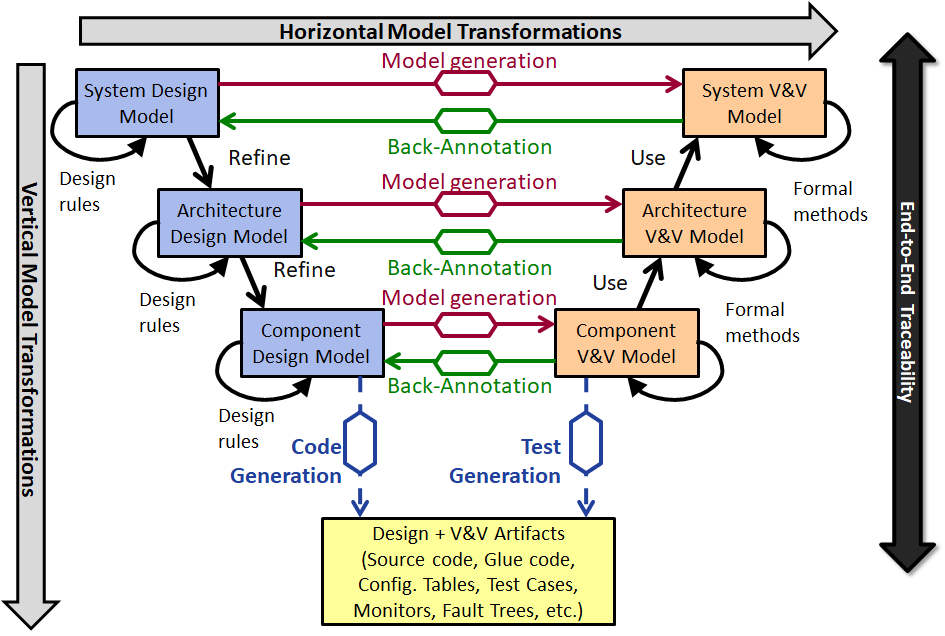
\includegraphics[width=.65\textwidth]{figures/mbse}
%\caption{Models transformations in model-based systems engineering}
%\label{fig:mbse}
%\end{figure}


Automated code generators (also called vertical MTs) improve productivity by synthesizing provenly correct source code of a safety-critical application from a validated model.% \cite{Sturmer-TSE2007}. 
In addition to source code generation, MBSE tools can synthesize other design artifacts (such as configuration tables, fault trees, test cases, documentation) and provide support for end-to-end traceability.% \cite{Aizenbud-IBMSystems-2006}. 
MBSE changes the traditional V-model of systems engineering into a Y-model where certain certification artifacts are synthesized automatically from models of proven quality used at different levels of abstraction.

%\subsection{Summary}
In Stage 1, my research was characterized by (1) proposing novel, foundational concepts, (2) developing innovative and scalable techniques, (3) architecting and maintaining cutting edge prototype tools based on solid foundations, (4) continuously benchmarking and empirically evaluating these tools, and (5) using these results at design time in a wide range of applications in tools used for engineering critical systems (like avionics and automotive). 

\subsection{Scalable incremental model queries: Techniques and tools}

\paragraph{Results.}
With my graduate students, G. Bergmann, M. Búr, Á. Hegedüs, Á. Horváth, G. Szárnyas, and I. Ráth, we developed highly scalable incremental techniques for continuously evaluating graph queries over large domain-specific instance models used in design and validation tools of critical systems. We turned scientific results \cite{models-2010-incquery,scp2015,models2014-iqd,icgt2015,sosym2016-viatra-invited} into mature scalable software tools, which instantly re-evaluate validation rules over domain-specific graph models with millions of elements. 

\paragraph{Impact.}
The \href{https://www.eclipse.org/viatra/}{VIATRA open source project} has been actively \emph{used at large companies and research institutes} (e.g. Thales, Airbus, Ericsson, ThyssenKruppPresta, Embraer, NASA JPL), and in \emph{industrial modeling tools} (e.g. Papyrus, Capella, Artop). It provides the basis of \emph{innovative products} (\href{https://incquerylabs.com/incquery/}{IncQuery for MagicDraw, IncQuery Server}) developed at IncQuery Labs Ltd. It has been \emph{regularly used a baseline in performance comparisons} by leading researchers (e.g. D. Kolovos, J. Cabot, H. Giese). I \emph{delivered several keynote talks} on related topics at major scientific conferences and summer schools. Related papers \cite{models-2010-incquery,icmt2011,ase2011-tool,ecmfa2011,models2014-iqd,scp2015,icgt2015,sosym2016-viatra-invited} have been cited over 400 times. 
% and \cite{models2018-tool} received a \textbf{Best Tool Paper Award} at the MoDELS 2018 conference. 

\paragraph{My role.}
All major contributors of the incremental graph query technology are my former PhD students. I have been the strategic leader of the research line until 2016 when the development of the open source framework was taken over by software engineers at IncQuery Labs Ltd, a high-tech company co-founded together with my former graduate students. This line of research has been funded by numerous national and international competitive research projects: I was the site leader at BME of \emph{collaborative European projects} (e.g. SENSORIA, SecureChange), and the principal investigator (PI) of an ERC Starting Grant application (CERTIMOT) which went to the final round, but became out of budget, and later it received partial funding from the Hungarian Research Agency (ERC-HU). 
%VIATRA technology received significant extra funding at IncQuery Labs, which is not detailed here. 


\subsection{Novel model transformations concepts}

\paragraph{Results.}
With my students, A. Balogh, Z. Balogh, G. Bergmann, Á. Hegedüs, Á. Horváth, I. Ráth, Z. Ujhelyi, we proposed novel model transformation concepts to capture mappings within and between various modeling languages. The scientific results provided foundations of the open source \href{https://www.eclipse.org/viatra/}{VIATRA} model transformation framework \cite{SCP2002,ASE2002,uml2004-meta,scp-2007,sosym2016-viatra-invited} which has been successfully developed along three generations since 2000. Novel concepts proposed by us for the first time include \emph{change-driven transformations} \cite{Rath-models09,sosym2011-cdt}, \emph{model transformation by example} (MTBE) \cite{models2006-varro,sosym2008-mtbe}, \emph{reactive transformations} \cite{icmt08-rbov08,icmt2015,sosym2016-viatra-invited} or \emph{model transformation slicing} \cite{ase2011-mtslice,icst2012}.

\paragraph{Impact.} 
In addition to its industrial use, we published our results on the VIATRA framework at major scientific venues of model-driven engineering including \cite{SCP2002,ASE2002,uml2004-meta,models2006-varro,scp-2007,Bergmann-icmt09,Rath-sosym09,Rath-models09,Bergmann-sttt10}, which have been cited well over 2000 times. The paper \cite{uml2004-meta} got the \textbf{10-year Most Influential Paper Award} at the IEEE/ACM MODELS 2014 conference (the main scientific forum of my research area), and I was invited to write an expert panel paper to the Software and Systems Modeling journal (SoSyM) \cite{sosym2016-viatra-invited}. Our first paper on change-driven transformations \cite{Rath-models09} received \textbf{Springer Best Paper Award} at IEEE/ACM MODELS 2009. The concepts of MTBE have been followed by 12 independent research groups worldwide. I delivered \emph{several keynote talks} at international conferences and summer schools on related topics.

\paragraph{My role.} 
The first open source version of VIATRA was developed by my graduate students, and I served as the strategic leader of the project until 2016 when development was taken over by IncQuery Labs Ltd. Therefore, I played key role in maturing a research prototype into an industrial framework. I was the main contributor (and hence, the first author) of the expert panel paper invited to the SoSyM journal.  I was the main supervisor of 5 PhD students and co-supervisor of 2 PhD students in addition to 20+ MSc students doing research and development on related topics. Co-founding IncQuery Labs enabled to keep together the core team for 15 years by now. I was the principal investigator (PI) of three IBM Faculty Awards, and an ERC-HU Starting Grant application and the site leader of various collaborative European projects (e.g. SENSORIA, SecureChange, MONDO) .

%My role in the related projects that funded this line of research is the same as in the previous line

\subsection{Performance benchmarks for model queries and transformations}
\paragraph{Results.}
Together with G. Varró and A. Schürr, we proposed the \emph{first performance benchmark for model transformation tools} in \cite{vlhcc05-vsv}. Since then, developing and maintaining performance benchmarks have been a focal topic of my research group. With my students, G. Bergmann, Á. Horváth, B. Izsó, G. Szárnyas, I. Ráth, Z. Ujhelyi, we systematically assessed the performance of various model query technologies \cite{Bergmann-sttt10,scp2015,ttc2015} of different modeling tools. 
%for different technological platforms along the Train Benchmark. 
In collaboration with researchers from University of Szeged, IncQuery was successfully used for detecting anti-patterns in source code of large projects \cite{csmr2014,ist2015}.

\paragraph{Impact.} 
Our first paper \cite{vlhcc05-vsv} triggered a series of annual Transformation Tool Contests (over 12 editions) and it received a \textbf{Most Influential Paper Award} at IEEE VL/HCC 2016. Moreover, \cite{csmr2014} received the \textbf{Best Paper Award} at CSMR-WCRE 2014. The Train Benchmark \cite{ttc2015} has been used by other researchers (e.g. D. Kolovos, X. De Carlos, G. Varró, G. Hinkel, H. Giese) for performance comparison from several independent research groups. Related papers have been cited over 275 times.

\paragraph{My role.} 
I was one of the three researchers who proposed the first benchmark for model transformations in 2005. 
%Benchmarking was a focal topic of my PhD student G. Szárnyas, while 
Later, I was a co-organizer of the first open transformation tool comparison as part of the AGTIVE 2007 conference \cite{agtive07-toolcontest}. My students (G. Bergmann, Á. Hegedüs, Á. Horváth, B. Izsó, I. Ráth, Z. Ujhelyi) made significant contributions to past benchmarking activities. I was the site leader at BME of the MONDO FP7 project, 
%and a collaborator in the MOGENTES FP7 project, 
which financed some of the related research activities.

\subsection{Rule-based guided design space exploration}

\paragraph{Results.}
Design space exploration (DSE) aims to derive design candidates fulfilling various design constraints from an initial design sketch by applying a pre-defined set of operations. We proposed the concept of \emph{rule-based guided design space exploration} \cite{Horvath-models09,sosym2011-csp,ase2011-dse,ause2015,ase2014,mpm2014} to incorporate complex structural consistency constraints frequently present in architecture models of automotive and avionics applications. The exploration process can be heuristically guided by hints obtained from the designer. DSE was applied to provide quick fixes in design environments built for business modeling \cite{vlhcc2011}. 

\paragraph{Impact.} 
Our paper \cite{ase2011-dse} at the IEEE ASE 2011 conference received an \textbf{ACM Distinguished Paper Award}. Other researchers (e.g. H. Vangheluwe, S. Zschaler and M. Wimmer) conducted research building on our results. Key papers \cite{Horvath-models09,vlhcc2011,sosym2011-csp,ase2011-dse,ause2015,ase2014} received over 150 citations in total. 
%The VIATRA-DSE open source software won \emph{two first prizes at the 9th Transformation Tool Contest} (TTC 2016). The prototype software was evaluated at NASA Jet Propulsion Lab for high-level mission planning.

\paragraph{My role.} 
DSE exploration served as a key research topic for three PhD students (Á. Horváth, Á. Hegedüs, A. Nagy) under my supervision, and I was last author in most of the key papers. Global search-based techniques were developed in collaboration with H. Sahraoui and H. Abdeen \cite{ase2014} during my period as a visiting professor at Université de Montréal in 2014. I was the site leader at BME of the DIANA EU project (which funded the initial investigations), and the PI of the CERTIMOT ERC-HU project and the research grant offered by Embraer (which funded subsequent investigations).

\subsection{Design techniques and tools for critical systems}

\paragraph{Results.} 
With my students, G. Bergmann, Á. Hegedüs, Á. Horváth, I. Ráth, Z. Ujhelyi, we developed novel techniques that can be used in design and verification tools used for safety-critical systems. \emph{Soft traceability links} \cite{models2012,sosym2016-trace} were developed within a collaborative project funded by Embraer (the large Brazilian airframer) to enable the seamless integration of models developed in different tools based on incremental model queries. 
We proposed a \emph{formal validation technique for domain-specific languages} \cite{models2013} in the same project to find inconsistencies in language specifications. The \href{https://github.com/viatra/massif/}{Massif} open source project interconnects of Matlab Simulink models and EMF-based modeling tools. 

\paragraph{Impact.} 
We published our results at top scientific venues of model driven engineering (e.g. MODELS conference, SoSyM journal). This line of research (started as part of the DIANA FP6 European project with large avionics companies) evolved into a 2-year \emph{collaborative industrial project funded by Embraer}, the large Brazilian aircraft manufacturer. As such, it had significant industrial impact. Our formal validation approach \cite{models2013} received \textbf{Springer Best Paper Award} at the IEEE/ACM MODELS 2013 conference. The Massif open source project has been used at several companies including Thales and MapleSoft.

\paragraph{My role.} 
I was the main supervisor of all the student contributors listed above, and consequently, I was the last author of most publications along this research line. I was the principal investigator of the collaborative project funded by Embraer, and I was the site leader at BME in the DIANA FP6 European project and the CONCERTO ARTEMIS project. I was a co-founder and Vice-President of Research and Development at OptXware Ltd., a start-up company founded at BME, which was partially acquired in 2013 by a large European company in the automotive domain. 
%An automotive design tool was developed at OptXware for a major tool vendor, which was a ke


\section{Recent Research Results: Stage 2 (2015- )}
\label{sec:recent-results-stage2}

\subsection{High-level overview of the research program}

\paragraph{Motivation.}
 A smart\& safe cyber-physical system (CPS) \autoref{fig:smart-safe-cps} is a software-intensive decentralized system that autonomously perceives its operational context and adapts to changes over an open, heterogeneous and distributed platform with a massive number of nodes, dynamically acquires available resources and aggregates services to make real-time decisions, and resiliently provides critical services in a trustworthy way. 
%Several challenges of such systems have been identified in \cite{Sztipanovits2012,Lee2014,Krupitzer2015,Cengarle2013,CPSoS2015}. 

In an open, interconnected and decentralized CPS, the components, the services, the underling execution platform and the environment may continuously evolve and change, thus distinction between design-time and run-time is blurred. %\cite{Baresi2010}. 
First, runtime information on services, platforms and deployment can be captured by runtime models %\cite{Blair2009,Szvetits2013} 
and operations on models will have direct effects on the running system. Then dynamic changes in requirements, services, resources, deployed configurations and reconfiguration rules need to be handled. Consequently, optimization and exploration will be pushed to runtime to guarantee that new deployment configurations do not jeopardize safety.

Recent advances in machine learning drives innovation in many sectors, e.g. to decrease energy consumption in smart buildings, to better adapt to current demands in smart factories or to prevent accidents in connected cars. But one needs to \emph{guarantee the trustworthiness of smart systems in a continuously evolving open environment}. It is a major challenge today for our society to prevent major future failures of such autonomous decentralized systems.

\begin{figure}
\centering
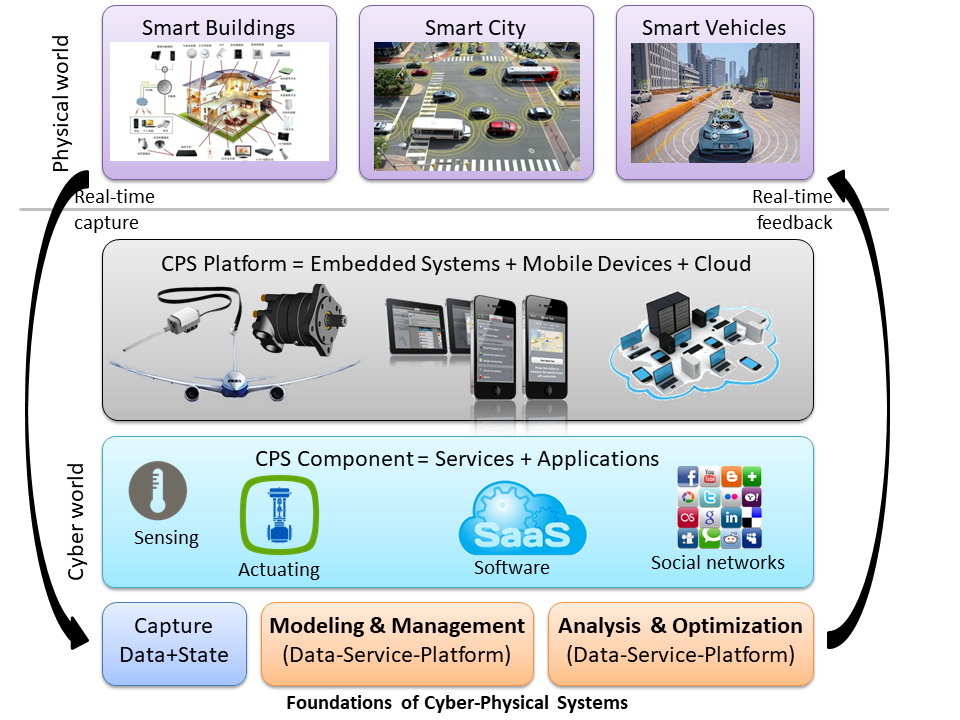
\includegraphics[width=.65\textwidth]{figures/smart-safe-cps}
\caption{Smart and safe cyber-physical systems}
\label{fig:smart-safe-cps}
\end{figure}


\paragraph{Objectives.}
My recent research has been aiming to develop innovative \emph{design, synthesis, management, validation and optimization techniques and tools}  for engineering smart and safe CPSs. In particular, my research group has been working to address two key long-term objectives:

\begin{itemize}
\item \textbf{Long-Term Objective 1}: How to \emph{design and manage} dynamically evolving smart\& safe CPSs to fulfill multi-domain requirements (e.g. consistency, extra-functional or physical)?
\item \textbf{Long-Term Objective 2}: How to \emph{guarantee or validate} that smart\& safe CPS with multi-domain requirements deliver quality of service in an open and changing environment?
\end{itemize}

%\paragraph{Research environment.}
%This research has been carried out in a rather unique and unconventional research environment. In 2015, I successfully acquired a Hungarian prestigious and highly selective Research Chair position funded by the Hungarian Academy of Sciences to run the \href{https://mta.hu/lendulet/az-mta-lendulet-kutatocsoport-halozata-105402}{MTA-BME Lendület Cyber-Physical Systems Research Group}. Here I was main supervisor of five PhD students, but I also provided co-supervision or strategic guidance for six other PhD students (partially affiliated to the project) who are supervised by young faculty members at the Department of Measurement and Information Systems. 
%In response to the increasing direct political influence on academic institutes and research funding imposed by the Orbán Government in Hungary, I joined the Department of Electrical and Computer Engineering at McGill University as a full professor in 2016. Since then, I have been coordinating research of a virtual (trans-Atlantic) group with frequent visits of Hungarian students at McGill.
%
%Furthermore, I was directly involved in strategically shaping proposals for European projects and training networks where IncQuery Labs Ltd was the involved partner.  Along these lines, we achieved the following major results in the past 5-6 years. 

\subsection{Distributed graph queries for runtime monitoring} 

\begin{table}[htb]
\footnotesize
\begin{tabular}{@{}p{5cm}p{11cm}@{}}
\toprule
%\textbf{ECSE 429 Questions} & \textbf{F18} \\ 
%\toprule
Publications &  \cite{sttt-2019-cps,fase2018-cps,wf-iot-2019,models2019-wcet} (all refereed), 1x \textbf{Best Paper Award} 
\cite{fase2018-cps} \\ \midrule
Graduate students at McGill & M. Búr, F. Khan \\ %\midrule
McGill undergraduates (SURE) &  C. Grosdidier \\ \midrule
%Past graduate students &  I. Ráth, Á. Horváth \\ \midrule
MTA-BME Lendület collaborators & A. Vörös \\ \midrule
%Other collaborators & G. Szilágyi, Z. Micskei, L. Balogh, B. Hegyi, B. Horváth, Z. Mázló \\ \midrule
%Key impact &  Publications at leading venues (including ICSE),  \\ \midrule
Funding &  NSERC DG (CA), MTA-BME Lendület (HU), NSERC Engage (under review) \\ %\midrule
\bottomrule
\end{tabular}
\caption{Summary: Distributed graph queries for runtime monitoring}
\end{table}

\paragraph{Motivation.} 
Since upfront formal verification is typically infeasible for smart CPSs, runtime monitoring is a common practice to continuously detect the violation of (safety) properties at runtime. Runtime monitoring has been addressed by runtime verification (RV) techniques %\cite{Leucker2009,Mitsch2014} 
which provide formal precision, but offer a low-level specification language (with simple atomic predicates to capture information about the system). 
%Recent RV approaches \cite{Havelund2015} started to exploit rule-based techniques over a richer (relational or graph-based) information model. 
Runtime models %\cite{BlairBF09,Szvetits2013} 
provide a rich knowledge representation to capture the runtime operational state and context of a smart CPS as typed and attributed graphs to serve as a unifying semantic basis for runtime assurance of self-adaptive systems (SAS).
%in \cite{Cheng2014,Vogel2014}. 
While graph models are widely used internally in various design tools for CPS (e.g. Capella, Artop), real-time CPSs dominantly use low-level data structures with static (i.e. compile-time) memory allocation to ensure resource constraints such as memory limits or deadlines, which is a major limitation.
% Unfortunately, \emph{such static data models are unable to capture dynamically evolving contextual information where there is no a priori upper bound on relevant contextual objects} (e.g. many pedestrians may be in contextual range of a self-driving car), which is a major limitation. 

\paragraph{Results.}
Together with my M. Búr (my PhD student at McGill), G. Szilágyi and A. Vörös, we proposed different graph-based technologies for runtime monitoring purposes in smart\& safe CPS, showcased in the context of the MoDeS3 research demonstrator \cite{nfm2018}. For that purpose, we adapted existing model management and distributed graph query techniques to be deployed over a heterogeneous, decentralized execution platform with resource constraints \cite{fase2018-cps}.  Since graph queries have traditionally been used at design-time by executing them on desktop computers (or servers), their adaptation to a resource-constrained runtime platforms is a highly complex challenge. 
We evaluated the performance of our graph query based runtime monitors \cite{wf-iot-2019} over the DDS (Data Distribution Service) platform, which is a standard of the Object Management Group (OMG). Furthermore, in a very recent journal paper \cite{sttt-2019-cps}, we precisely formalized the behavior of our distributed algorithms and carried out a more extensive scalability evaluation. 
In order to use such graph query techniques for monitoring purposes in hard real-time applications, the worst case execution time (WCET) of the monitoring programs needs to be estimated. Thus in our recent MODELS 2019 paper \cite{models2019-wcet}, we proposed a long-term research agenda and an initial approach that exploits existing WCET analysis tools for calculating WCET for graph queries.

\paragraph{Impact.} 
We published several papers at leading conferences  \cite{fase2018-cps,models2019-wcet} and journals \cite{sttt-2019-cps}. Our paper \cite{fase2018-cps} received an \textbf{EASST Best Paper Award} at ETAPS 2018 (1 award out of over 140 papers). The MoDeS3 framework has been demonstrated at numerous industrial and other public events at BME (e.g. at the annual Researchers Night). These conceptual results have been successfully used in the MoDeS3 open demonstrator for smart and safe CPSs \cite{nfm2018}. I delivered a keynote talk at Ericsson Industrial Day 2016, at the CSCS 2016 Hungarian conference for PhD students, and several invited lectures at the DSM-TP international summer school in several consecutive years. Our results will provide a basis for an upcoming industrial collaboration with Predikat Inc. (Canada) where runtime monitoring of performance degradations in multi-tier web applications will be carried out (the NSERC Engage project is still under review).
% and in an initial prototype developed for the successful Hungarian start-up TeqBall.

\paragraph{My role.}
I was the strategic initiator of this line of research. I was also the main supervisor of M. Búr (PhD student at McGill) and provided strategic guidance for A. Vörös (assistant professor at BME). I contributed to the precise mathematical formulation of the results \cite{fase2018-cps,sttt-2019-cps,models2019-wcet} and also to the textual contents of all publications. I was the PI of a related NSERC Discovery Grant (Canada), an NSERC Engage application and the Lendület Research Group (Hungary). 

\subsection{Automated generation of domain-specific graph models: The CORE-DISC challenge}

\begin{table}[htb]
\footnotesize
\begin{tabular}{@{}p{5cm}p{11cm}@{}}
\toprule
%\textbf{ECSE 429 Questions} & \textbf{F18} \\ 
%\toprule
Publications &  \cite{fmhe2018,sosym2017-dsl,sttt-2019-div,fase2018-diverse,fase2016-solver,icse2018-solver,icse2019-tool,MODELS2016-metrics,MODELS2016-bx,models2018} (all refereed), 2x defended PhD theses (by O. Semeráth, G. Szárnyas) \\ \midrule
Graduate students at McGill & A. Babikian \\ %\midrule
Graduate research trainees at McGill &  O. Semeráth, G. Szárnyas (PhD students defended at BME, supervisor), K. Marussy (PhD student at BME, co-supervisor)  \\ %\midrule
McGill undergraduates (SURE) &  A. Babikian, S. Pilarski, A. Li, B. Chen, L. Li, M. Ding, V. Gidla \\ \midrule
Past graduate students &  G. Bergmann, Á. Horváth \\ \midrule
MTA-BME Lendület collaborators & R. Farkas, A. Vörös \\ \midrule
Other collaborators & Z. Szatmári \\ \midrule
%Key impact &  Publications at leading venues (including ICSE),  \\ \midrule
Funding &  NSERC DG (CA), MTA-BME Lendület (HU) \\ %\midrule
\bottomrule
\end{tabular}
\caption{Summary: Automated generation of domain-specific graph models}
\end{table}

\paragraph{Motivation.}
Graphs are key abstractions in science and engineering. They may represent linked data in graph databases, complex designs of cyber-physical systems or critical contextual situations for autonomous systems. Synthetic graph generators are essential when the use of real graph models is restricted (to respect privacy regulations or intellectual properties of companies) or impractical (to find corner-cases for safety assurance). I initiated the CORE-DISC \emph{long-term research program program} \cite{fmhe2018} to develop a next generation of synthetic graph generator techniques and tools that are customizable to different application domains to derive graph models which are simultaneously \emph{CO: consistent} (graphs shall satisfy various structural logic constraints of the domain), \emph{RE: realistic} (synthetic graphs shall resemble real graphs of a given domain), \emph{DI: diverse} (any pair of graphs shall be structurally distant from each other) and \emph{SC: scalable} (the graph generator shall be able to derive large graph models). Such synthetic graphs are intended to be used as test cases in tool qualification process prescribed by safety standards.% (like DO-330).

\paragraph{Results.} 
As consistency appeared to be the most difficult property to achieve, our initial investigations \cite{fase2016-solver,sosym2017-dsl} aimed to derive consistent graph models with the use of existing logic solvers like Alloy with Kodkod (from MIT) 
%\cite{Torlak2007} 
or Z3 (from Microsoft Research) %\cite{Moura-tacas2008}, 
but none of these attempts were able to scale by failing generate models with over 100 graph nodes. Therefore, we developed a novel \emph{consistent graph solver} \cite{icse2018-solver,icse2019-tool}(with my students, O. Semeráth, A. Nagy, G. Szárnyas, A. Babikian and S. Pilarski) for automatically generating consistent graph models by implementing a novel refinement calculus over partial models \cite{fmhe2018} and using an approximation technique based on constraint rewriting \cite{icmt2017}. Our consistent graph solver \cite{icse2018-solver,icse2019-tool} scales 1-2 orders of magnitude better than competitors that use background logic solvers and its scalability is comparable to search-based techniques %\cite{Soltana2017} 
while uniquely providing both consistency and completeness guarantees. We successfully applied the model generator for incremental backward propagation of view models \cite{MODELS2016-bx} as well as for incremental view model synchronization \cite{models2018}.

Moreover, we provided the first characterization of \emph{realistic models} in \cite{MODELS2016-metrics,fmhe2018} by adapting various graph metrics from network science and evaluating them on graph models taken from six different domains of software and systems engineering. By adapting graph shapes, %\cite{Rensink}, 
we proposed various \emph{model diversity metrics} \cite{fase2018-diverse,sttt-2019-div} by which generalize and subsumes several existing coverage metrics used for testing of model transformations. We extended our model generator and showed that it derives more diverse models than its direct competitors \cite{fase2018-diverse,fmhe2018,sttt-2019-div}. 

%aimed  Generating consistent After a series of initial results , we rea attempts with negative scalabil results 

\paragraph{Impact.}
We published our results in a series of papers at leading conferences and journals of software engineering including 1 book chapter, 1 journal paper at SoSyM \cite{sosym2017-dsl}, 1 at \cite{sttt-2019-div} in Software Tools on Technology Transfer (Springer), 2 papers at MODELS \cite{MODELS2016-bx,models2018}, 2 papers at FASE \cite{fase2016-solver,fase2018-diverse}. I also two invited talks on this topic: one at the CSER 2017 conference in Montreal and one at the Search Based Model Engineering Workshop at King's College London in 2018.
As a special highlight, we published a research paper \cite{icse2018-solver} and a tool paper \cite{icse2019-tool} at ICSE, the prime general-purpose software engineering conference, which is a major success as no modeling papers had been published in the previous three editions of ICSE. 
The news about our ICSE paper \cite{icse2018-solver} was \emph{featured on the front page of the Hungarian Academy of Sciences} (\href{http://mta.hu/english/innovation-of-hungarian-researchers-could-revolutionise-car-industry-design-technology-testing-108434}{Eng}, \href{http://mta.hu/tudomany_hirei/magyar-kutatok-eredmenye-forradalmasithatja-az-autoipari-tervezoeszkozok-teszteleset-108355}{Hun}) and shared by \emph{six major news portals in Hungary}, and I received three invitations for interviews in radio channels. 
%Our approach (published in \cite{sosym2017-dsl,act2017,fmhe2018,fase2018-diverse,icse2018-solver,icse2019-tool}) \emph{scales 1-2 orders of magnitude better} than competitors using state-of-the-art logic solvers like Alloy (MIT) or Z3 (Microsoft Research) and its scalability is comparable to search-based techniques \cite{Soltana2017}. 

%The model generator tool \cite{icse2018,icse2019-tool} provides 1-2 orders of magnitude better scalability compared to exis
%Already the initial results for the formal validation technique for DSLs \cite{models2013} (extended later to the journal paper \cite{sosym2017-dsl}) received Best Paper Award at the IEEE/ACM MODELS 2013. 

\paragraph{My role.}
I was the sole PhD supervisor of key contributors (O. Semeráth, G. Szárnyas, A. Nagy) and MEng students (A. Babikian, S. Pilarski) of this research line, hence being the last author in all papers above. I was the first author of \cite{fmhe2018}, which presents a long-term research agenda and challenges for automated graph model generation. My technical contributions  include some precise foundations and key theorems for the refinement calculus over partial models. I was the PI of the Lendület project and NSERC Discovery Grant that provided funding for the involved students.


\subsection{Secure collaborative modeling}

\begin{table}[htb]
\footnotesize
\begin{tabular}{@{}p{5cm}p{11cm}@{}}
\toprule
%\textbf{ECSE 429 Questions} & \textbf{F18} \\ 
%\toprule
Publications &  \cite{sosym2017-mondo,ieeesw2018,MODELS2016-access,fase2016-merge,esec-fse2017,%
models2017,vlhcc2018,commitmde2016,commitmde2017} (all refereed), 1x PhD thesis (under review), 
1x \textbf{Distinguished Paper Award} \cite{MODELS2016-access}
\\ \midrule
Graduate students at McGill & M. Búr  \\ %\midrule
Graduate research trainees at McGill &  C. Debreceni (PhD student at BME, main supervisor) \\ \midrule
Past graduate students &  G. Bergmann, I. Ráth \\ \midrule
Other collaborators &   De Carlos, X. Mendialdua and S. Trujillo (Ikerlan, Spain), A. Barisic, V. Amaral, M. Goulao (Nova Univ. Lisbon, Portugal) \\ \midrule
Funding &  MTA-BME Lendület (HU), MONDO (EU), NSERC DG (CA), %Bolyai scholarship (HU, secured by G. Bergmann)
 \\ %\midrule
\bottomrule
\end{tabular}
\caption{Summary: Secure collaborative modeling}
\end{table}

\paragraph{Motivation.}
As a common industrial practice in model-based systems engineering, system integrators frequently outsource the development of various components to subcontractors in an architecture-driven supply chain where the collaboration between cross-organizational teams is facilitated by sharing models stored in model repositories. However, effective cross-organizational collaboration is hindered by numerous factors, such as (1) lack of appropriate fine-grained access control management to protect the intellectual property rights (IPR) of involved parties, (2) model fragmentation, or (3) the inability to combine online (GoogleDoc type) and offline (Git or SVN-like) collaboration schemes. 

\paragraph{Results.} 
Together with C. Debreceni, M. Búr, G. Bergmann and I. Ráth, we developed a collaborative modeling framework \cite{esec-fse2017,ieeesw2018} that enhances modeling repositories by providing secure views as an extra protection layer with rule-based high-level access control simultaneously enforced for both offline and online collaboration scenarios and adapted to software configuration management. As a novel underlying concept, we developed a rule-based fine-grained access control technique using bidirectional transformations \cite{MODELS2016-access}. The soundness of the core collaboration scheme was formally proved and successfully applied for both online and offline collaborations in \cite{sosym2017-mondo}. 
Further technical details about the fine-grained model-level access control were published in two peer-reviewed workshop papers \cite{commitmde2016,commitmde2017}. 
To enhance the practical usefulness of the collaborative modeling framework, we developed an automated model merge technique driven by design space exploration \cite{fase2016-merge} (which was evaluated in a collaborative user study \cite{vlhcc2018}). Furthermore, we successfully developed an approach \cite{models2017} to implement the concepts of property-based locking that prevents unintentional model modifications during extensive collaboration. 

\paragraph{Impact.} 
We published seven research papers \cite{fase2016-merge,MODELS2016-access,models2017,esec-fse2017,vlhcc2018,sosym2017-mondo,ieeesw2018} at leading scientific forums (including conferences like MODELS, FASE, ESEC/FSE, VL/HCC and journals like Software and Systems Modeling and IEEE Software). Paper \cite{MODELS2016-access} received \textbf{ACM Distinguished Paper Award} at the MODELS 2016 conference, while the papers above received over 40 citations (Google Scholar). Related concepts were integrated into an innovative product developed by IncQuery Labs Ltd. \cite{models2018-tool}.
%Paper \cite{vlhcc2018} carried out a user study in an industrial setting as part of the MPM4CPS EU COST Action.

\paragraph{My role.} 
I was the strategic initiator of this research line, thus the last author in most related publications (except for the collaborative paper \cite{vlhcc2018}). I am the main supervisor of C. Debreceni and M. Búr who were major technical contributors of the framework. C. Debreceni has already submitted his PhD thesis, and his public defense is expected in Fall 2019. I was the site leader of the MONDO FP7 project at BME where this line of research was started, and the PI of the Lendület project which provided continuity. I helped G. Bergmann (who is an assistant professor at BME) to successfully apply to the prestigious János Bolyai Scholarship in Hungary in a related research topic. 

\subsection{Platform for digital multidisciplinary analysis and design optimization}

\begin{table}[htb]
\footnotesize
\begin{tabular}{@{}p{5cm}p{11cm}@{}}
\toprule
%\textbf{ECSE 429 Questions} & \textbf{F18} \\ 
%\toprule
Publications &  \cite{mdeintelligence2019} (refereed), 3x MEng thesis (in preparation) \\ \midrule
Graduate students at McGill & M. Rangappa, J. Dhaliwal \\ \midrule
Other collaborators &  M. Staniszewski, Frederic Villeneuve (and other Siemens engineers) \\ \midrule
Funding &  NSERC CRD with Siemens (CA) \\ %\midrule
\bottomrule
\end{tabular}
\caption{Summary: Digital multidisciplinary analysis and design optimization platform}
\end{table}

\paragraph{Context.}
Gas turbines are a commonly used type of internal combustion engine used for power generation. The development of gas turbines requires creation of many different linked models by mechanical engineers. These models are used in gauging performance, designing secondary air systems, combustion, and other subsystems. Creation of design models can span across dozens of design tools which can integrate many data formats, disciplines, and requirements, which introduces significant software engineering challenges. For example, the large number of models inherently results in a huge design exploration space during the development process of an entire engine. Furthermore, the actual tool workflows need to be seamlessly integrated with the underlying development processes.

\paragraph{Results.}
This industrial CRD project started in 2018, and we work on innovative software-as-a-service solutions to integrate various design, analysis and optimization tools driven by workflows. This line of research is carried out together with my McGill MEng students, Maruthi Rangappa, Jasvir Dhaliwal and Sebastian Pilarski, and in collaboration with leading Siemens managers (M. Staniszewski and F. Villeneuve). We aim to develop a cloud-based solution to systematically store and query simulation results to allow fast iterations and a more agile design process. Moreover, we aim to exploit advance machine learning techniques to bring expertise gained from field data and simulated data directly to the mechanical engineers working on engine design. Initial results and a research roadmap has been proposed in \cite{mdeintelligence2019}, while two MEng theses about a graphical workflow editor and an "analysis tool as a service" infrastructure are planned to be submitted by J. Dhaliwal and M. Rangappa in Fall 2019.

\paragraph{Impact.}
While the project is still in an early phase, we made significant technological impact within Siemens. A software prototype developed by Sebastian Pilarski's will serve as the baseline software architecture for a cloud-based simulation environment being developed at Siemens. We also published a joint vision paper with leading Siemens managers at a MODELS 2019 workshop \cite{mdeintelligence2019}. 

\paragraph{My role.}
I am a co-PI of the NSERC project (PI: M. Kokkolaras - McGill, co-PI: H. Moustapha - ETS), and the only software engineering professor in the collaboration. I was contributing to the entire project preparation and proposal writing phase. I am the main supervisor of the three MEng students working on the project. In 2018, I was an invited speaker at the Siemens Industrial Day at ETS (Montreal), and also gave a talk about the project for graduate students.


\subsection{Continuation of previous research lines}
\paragraph{Results.} 
Naturally, I also continued previous research lines started in Stage 1 of my career. Below I summarize and report results where major progress has been made after I joined McGill University. 

\begin{itemize}[leftmargin=0.5cm]
\item
\textbf{Benchmarks for incremental graph queries:}
With key contributions from G. Szárnyas (my PhD student), we prepared a journal paper \cite{sosym2017-tb} to extend the Train Benchmark with a cross-technology comparison of graph query techniques with over 10 tools (including relational databases, graph databases, Eclipse-based modeling tools, rule-based expert systems, etc.). Thanks to the free availability of its source code repository, the Train Benchmark has been actively used by four independent research groups within the model-driven engineering community.


\item 
\textbf{Model transformation techniques:}
Together with O. Semeráth, C. Debreceni (my PhD students), K. Marussy (co-supervised by me) and Á. Horváth, we published two papers at the MODELS conference about the incremental backward synchronization of model transformations \cite{MODELS2016-bx} and fully incremental view model transformations \cite{models2018}. 

\item
\textbf{Design space exploration:}
Thanks to the key contributions from my PhD students, A. Nagy and O. Semeráth, the VIATRA-DSE open source software won \emph{two first prizes at the 9th Transformation Tool Contest} (\href{https://www.transformation-tool-contest.eu/2016/solutions_cra.html}{TTC 2016}). Subsequently, the prototype software was evaluated at NASA Jet Propulsion Lab for high-level mission planning.

\item
\textbf{Formal verification of reactive systems:}
With V. Molnár, Á. Hajdu (graduate research trainees at McGill), B. Graics, A. Vörös, Z. Micskei, I. Majzik (staff members at BME and main supervisors of PhD student), we developed a high-level modeling language for semantically precise composition of reactive components defined by statecharts where each component may follow a different execution semantics (e.g. synchronous vs. asynchronous). The Gamma tool was demonstrated at ICSE 2018 \cite{icse2018-gamma} and the related research paper \cite{sosym-2019-gamma} is under review. I gave an invited talk and a tutorial about this line of research at the DSM-TP 2017 international summer school.


\end{itemize}


\subsection{International research collaborations}

While as a senior researcher, my main mission is to supervise graduate students and help them mature as independent researchers, I still continue participating in international collaborations that typically result in joint publications. Below I summarize a few joint initiatives from the past 3-4 years. 

\begin{itemize}[leftmargin=0.5cm]
\item \textbf{Server-side incremental queries } 
I actively collaborated with researchers and software engineers of IncQuery Labs Ltd. from the inception phase to develop an innovative, server-side product called IncQueryServer for TeamWork Cloud. The product exploits advanced graph query techniques to provide cloud-based server-side validation services over large system models captured in the standard SysML language. The product is  provided as an add-on to a popular cloud-based model repository product of NoMagic/Dassault Systems. We published a joint tool demonstration paper \cite{models2018-tool}, which  received a \textbf{Best Tool Paper Award} at the MODELS 2018 conference.

\item \textbf{Survey on model transformations} In 2017, I was invited to collaborate on a new survey assessing the state of the art of model transformation tools with N. Kahani, M. Bagherzadeh, J. Cordy and J. Dingel (all from Queen's University). The collaboration resulted in a joint paper \cite{sosym2019-mt} published at the SoSyM journal in 2019 and it already received 10+ independent citations.

\item \textbf{Complex event processing for runtime models}
As a continuation of past research \cite{models2014-stream} carried out with I. Dávid (Univ. Antwerp, Belgium) and I. Ráth to adapt the concepts of complex event processing for runtime models for stream processing, we published an extended journal version of our results which contained precise formalization of our concepts \cite{sosym2018-cep}. Certain concepts along this line were used in a proof-of-concept prototype developed for the successful Hungarian start-up TeqBall.

\item \textbf{User study on model merge techniques} 
Together with A. Barisic, V. Amaral, M. Goulao (researchers at Nova Univ. Lisbon, Portugal) and my PhD student C. Debreceni, we collaboratively carried out and published a user study \cite{vlhcc2018} to assess the usability of a novel model merge technique. In fact, the model merge technique \cite{fase2016-merge} was also a result of collaborative research within the MONDO project with X. De Carlos, X. Mendialdua and S. Trujillo (from Ikerlan, Spain). The execution of user study was mainly driven by the collaborators from Portugal (and partially supported by MPM4CPS EU COST Action), while we provided technical support for the focal tool of the user study. 
\end{itemize}


\section{Future Research}

%\subsection{Context}

\paragraph{Motivation.} 
Digitalization is a dominating trend in engineering in initiatives like Industry 4.0 or Internet-of-Things. The concept of \emph{digital twins} (i.e. digital replica of physical assets, processes, people, places, systems) requires developing and continuously maintaining a digital representation of design documents in the form of models using a multitude of design, validation and optimization tools. The traditionally separate design and operation phases are blurred by systematically recording operational (field) data and processing it by machine learning and software engineering techniques to provide useful input for next design cycles. Decision making in autonomous CPSs (like self-driving cars, or drones) relies upon runtime models collected by a network of sensors, and fused by various artificial intelligence techniques. 

\paragraph{Main challenge.}
While innovation for digitalization is driven by software and intelligent data processing techniques; however, there is too much optimism for their fast penetration to critical CPSs (like cars, aircrafts, space) while appropriate means of quality assurance is severely lacking, especially in the presence of an increased level of automation or autonomous behavior.
 
%\begin{itemize}
%\item[(1)] 
While dozens of software tools are necessitated to a fully digital design of a complex CPS, quality assurance for tools and integrated tool chains is insufficient and represents a major risk for digitalization. How to trust a digital twin if one cannot trust the software tool used for designing it? Software safety standards of critical avionics systems (\href{https://standards.globalspec.com/std/1461615/rtca-do-330}{DO-330}) prescribe that only the output of a qualified tool can be trusted, and such a tool should meet the same requirements as the critical system component it designs. However, it makes tool qualification extremely costly.

%\item[(2)]
Due to recent fatal accidents, the safety assurance of autonomous cyber-physical systems (like self-driving cars or autonomous drones) is still its infancy. Unfortunately, decades of verification and validation (V\&V) practices developed for traditional safety-critical software systems are not applicable to autonomous systems. Existing practices rely up exhaustive simulation for system validation, but statistical techniques do not provide sufficient level of dependability and coverage in case of extremely rare events where one combination of rare events may jeopardize safety.
%\end{itemize}

\paragraph{Objectives.}
As a high-level objective, my ongoing and future research aims to increase the level of trust in digitalization for CPSs by developing systematic validation techniques for design tool chains and autonomous systems by automatically synthesizing potentially unsafe or problematic corner-cases and contextual situations. While the potential of digitalization is unquestionable, this project will mitigate its risks and negative impacts.

In particular, I am interested in novel scientific foundations and scalable software tools for 
\begin{enumerate}
\item the integration and testing of design tools used in digitalization for CPS, 
\item the system-level assurance of autonomous CPS,
\item the systematic testing for intelligent CPS driven by machine learning. 
\end{enumerate}

\paragraph{System-level assurance of autonomous CPS}
%\paragraph{Key ideas.}
Since safety-critical autonomous vehicles need to interact with an immensely complex and continuously changing environment, their assurance is a major challenge, and upfront design time assurance is generally regarded to be practically infeasible. While systems engineering practice necessitates assurance on multiple levels,  existing research focuses dominantly on component-level assurance while neglecting complex system-level traffic scenarios.
Our research aims to address the system-level testing of the situation-dependent behavior of autonomous vehicles by combining various model-based techniques on different levels of abstraction. Major initial progress and a research roadmap (developed in a SURE project in Summer 2018 and later in collaboration with researchers from BME but still under my scientific leadership) is reported in a vision paper \cite{models2019-systest} accepted at the MODELS 2019 conference.

%(1) Safety properties are continuously monitored in challenging test scenarios (obtained in simulators or field tests) using graph query and complex event processing techniques.  (2) To precisely quantify the coverage of an existing test suite with respect regulations of safety standards, we provide qualitative abstractions of causal, temporal, or geospatial data recorded in individual runs into situation graphs, which allows to systematically measure system-level situation coverage (on an abstract level) wrt. safety concepts captured by domain experts.  (3) Moreover, we can systematically derive new challenging (abstract) situations which justifiably lead to runtime behavior which has not been tested so far by adapting consistent graph generation techniques, thus increasing situation coverage. (4) Finally, such abstract test cases are concretized so that they can be investigated in a real or simulated context.

%\begin{enumerate}
%\item Safety properties are continuously monitored in challenging test scenarios 
%(obtained in simulators or field tests) using graph query and complex event processing techniques.  
%\item To precisely quantify the coverage of an existing test suite with respect regulations of safety standards, we provide qualitative abstractions of causal, temporal, or geospatial data recorded in individual runs into situation graphs, which allows to systematically measure system-level situation coverage (on an abstract level) wrt. safety concepts captured by domain experts. 
%\item Moreover, we can systematically derive new challenging (abstract) situations which justifiably lead to runtime behavior which has not been tested so far by adapting consistent graph generation techniques, thus increasing situation 
%coverage. 
%\item Finally, such abstract test cases are concretized so that they can be investigated in a real or simulated 
%context.
%\end{enumerate}

%\subsection{Testing of data sets used for machine learning in CPS design}
%
%\paragraph{Objectives.} Even when a large amount of field data is available as a training set, machine learning techniques provide no guarantees that this training set covers particular corner cases and rare events. We plan to devise an iterative and incremental approach which continuously evaluates a training set with respect to some coverage criteria over an abstract (graph-level) equivalence class, and then uses a graph generator (see below) to systematically derive test data for uncovered partitions of training data.
%
%\subsection{Auto-generation of consistent, realistic, diverse and scalable models}
%\paragraph{Objectives.} As a cross-domain underlying research line, we aim to develop automated synthetic graph generators with precise foundations, efficient algorithms and open-source scalable software prototype implementation to derive domain-specific graph models which are \emph{simultaneously consistent, realistic, diverse and scalable}. 
%Since graphs provide key abstractions of complex information in science and technology (including  design and runtime information of complex, software-intensive CPS), auto-generated graph models can serve as test cases or benchmarking purposes, especially, in data intensive, decentralized applications.

\section{Research Funding}

\subsection{Past research funding (Stage 1)}
In the first stage of my career, I was successful in attracting a variety of substantial research funding with both individual and collaborative research projects, with academic as well as industrial funding. 

\paragraph{Collaborative European projects: }
Since 2005, I was the site leader or research coordinator at BME for a series of collaborative European projects. The \emph{SENSORIA project} (2005-2010) aimed to provide precise software engineering techniques for next-generation service-oriented overlay computers. The \emph{DIANA project} (2006-2010) involved large avionics companies to provide a distributed and equipment-independent environment for avionics applications compliant with the ARINC 653 standard. The E-Freight project (2010-2013) aimed to improve on European e-freight capabilities for combined transport routes. The SecureChange project (2009-2012) developed various security engineering techniques used for evolving software-intensive systems. Finally, the MONDO project (2013-2016) was concerned with the development of scalable modeling and model management techniques deployed over a cloud platform.
I was involved in these projects starting both during the proposal writing as well as the actual execution phase. I was the scientific leader for different work packages, coordinated the development of project demonstrators, and altogether, I successfully collaborated with well over 100 researchers in Europe.

\paragraph{Individual research grant applications: }
I was also successful in grant applications where I was the sole PI. In particular, my ERC Starting Grant project (CERTIMOT: Design and Analysis Techniques for Certifiable Model Transformations) went to the final round of reviews at the European Commission with a supportive score of 7/8, but it became out of budget. Finally, it received partial funding from the Hungarian Research Agency and ran between 2010 and 2014. My application to the MTA Lendület research chair program is detailed below.


\paragraph{Industrial funding: }
I was the principal investigator of a two-year research project (TRANS-IMA) funded by Embraer, the large Brazilian airframer to develop innovative model-based avionic tools for their systems engineering process (total funding: 200,000 EUR). Previously, I was the three times recipient of the IBM Faculty Award offered by IBM TJ Watson Research Center (total amount of 36,000 USD). I was research coordinator for two collaborative projects with Nokia Research Centre (Budapest) on high-availability service platforms and model-driven development techniques (approx. 40,000 EUR).

\subsection{Recent research funding (Stage 2)}
Since 2015, I successfully continued to secure substantial amount of research funding with a total amount of Canadian funding over 1.46 million CAD as PI or co-PI (own share of funding: 580,000 CAD), and additional own funding over 160 million HUF (equivalent of over 730,000 CAD) in Hungary. Except for my start-up grant offered by McGill University, all other grants were secured on a competitive basis. Further financial details of funding are listed in my CV.

\paragraph{NSERC CRD: Digital Multidisciplinary Analysis and Design Optimization Platform (2018-2023): }
We started a 5-year long multidisciplinary collaborative research and development (CRD) project co-funded by Siemens Canada and NSERC targeting a design platform for designing aeroderivative gas turbines. The total funding of the project is around 1.2 million CAD (with roughly 25\% is reserved to my own research). 

%Furthermore, I gave two invited talks at the Siemens-ETS Industry 4.0 Day in Montreal in 2018. 

\paragraph{NSERC Engage (2019-2020): Automated identification of performance regressions in a multi-tier web applications, under review}
With its innovative Predicate AIOps tool suite, our industrial partner, Predikat Inc. offers innovative solutions to prevent down-time and predict traffic for multi-tier web applications for companies providing business-critical
Software-as-a-Service solutions deployed over virtual machines or as microservices using a complex,
multi-layered software stack composed of heterogeneous technologies. As a specific problem at Predikat,
finding the root cause of identified performance regressions is a time-consuming manual task. This project
aims to identify performance bottlenecks in multi-tier web applications by runtime monitoring and then provide
automated root cause analysis to trace the bottleneck to the relevant component in real-time, thus removing the
burden of manual troubleshooting from DevOps engineers. As such, it would further enhance the existing
capabilities of the Predicate AIOps tool suite. The project is under evaluation, and it is expected to run for six months starting in Fall 2019.

\paragraph{NSERC Discovery Grant (2016-2021): Model-based Design and Validation Techniques for Smart and Safe
Cyber-Physical Systems:}
Due to its flexible nature, my NSERC Discovery Grant provided funding for students without having an industrial project. This included Márton Búr (PhD student at McGill), and Faizan Khan (MEng student at McGill) to carry out research in the context of Internet-of-Things applications of cyber-physical systems. In addition, it funded a total of 9 undergraduate students who participated in early research activities as part of the Summer Undergraduate Research in Engineering (SURE) program. Furthermore, travel costs of several Hungarian PhD students who visited my as McGill graduate research trainees were covered.

\paragraph{LiveIDE: Live Integrated Development Environment for Software-Intensive Communication Systems (2017): }
In 2017, I led the submission of a proposal as principal investigator for a three-year NSERC Strategic Partnership Grant for Projects with G. Mussbacher, J. Kienzle (McGill), H. Sahraoui and E. Syriani (UdeM) as co-PIs and Ericsson Montreal as supporting industrial partner. NSERC offered to accept the project without further changes as a collaborative research and development (CRD) project due to its industrial relevance, but unfortunately, this CRD contract was not signed as the main contact and project lead at Ericsson left the company (after 20 years).

\paragraph{MTA-BME Lendület Cyber-Physical Systems Research Group (2015-2020)}
This prestigious and highly selective research chair program is run by the Hungarian Academy of Sciences, and each year a total of 12-15 researchers below the age of 45 are awarded nation-wide. In 2015, I was only the third ever recipient in the field of computer science. The project provided partial funding for 10 PhD students and 2 junior staff members at BME to do research on various challenges of cyber-physical systems.

%\paragraph{Further initiatives for research funding:}
%In addition, I was actively seeking further opportunities for research funding, being the PI for a proposal for the 
%MSSI (McGill Sustainability Systems Initiative) Ideas fund (Sustainity: A Knowledge Base for Sustainability Research) with G. Mussbacher (McGill) as co-PI, and being the co-PI in in an application submitted in the NSERC Collaborative Research and Training Experience (CREATE) program (TRANSMIT: Training program in continuous software migration to emerging technologies), and a co-PI in a proposal for the IDEaS Innovation for Defence and Security Program (Enhanced Human-Robot Collaboration with Wearable Technology) with G. Beltrame (Polytechnique), A.M. Cretu (Carleton), E. Coffey (Concordia) as PIs. Unfortunately, these initiatives did not receive funding in the respective competitions. 

%\newrefcontext{extref}
%\printbibliography[heading=subbibliography,notcategory=own,title=External references]
